\PassOptionsToPackage{authoryear,round}{natbib}
\documentclass[11pt,twocolumn]{article}
\usepackage{report}

\usepackage{hyperref}       % hyperlinks
\usepackage{url}            % simple URL typesetting
\usepackage{booktabs}       % professional-quality tables
\usepackage{amsfonts}       % blackboard math symbols
\usepackage{nicefrac}       % compact symbols for 1/2, etc.
\usepackage{microtype}      % microtypography
\usepackage{graphicx}
\usepackage{amsmath}
\usepackage{titling}
\usepackage{caption}
\usepackage{subcaption}
\captionsetup{labelsep=period}
%\usepackage[font=small]{caption}
\setlength{\droptitle}{-20pt}  % Adjust as needed


\usepackage{amssymb}
\usepackage{pifont}
\newcommand{\cmark}{\checkmark}
\newcommand{\xmark}{\ding{55}}

\usepackage{titlesec}



\title{\vspace{-1em}{\Large\textbf{Garment Texture Completion in UV space using Stable Diffusion}}\vspace{-1em}}

\author{
  \begin{tabular}{c c}
  Ludek Cizinsky & Yingxuan You\thanks{Yingxuan contributed the initial research idea and the foundational model pipeline, building on her prior work. Throughout the semester, she provided Ludek with valuable guidance and constructive feedback.}  \\
  \texttt{ludek.cizinsky@epfl.ch} & \texttt{yingxuan.you@epfl.ch} \\
  EPFL & EPFL
  \end{tabular}
}


\begin{document}

\date{}
\maketitle



\begin{abstract}
\textit{We present a method for completing garment texture maps in UV space using a diffusion 
model conditioned on masked input and text prompts. Our approach focuses on 
predicting diffuse textures as a first step toward high-fidelity, 
physically based rendering (PBR) of garments. To train our model, we construct a synthetic 
dataset of 27,000 garment textures with corresponding PBR maps generated using the 
DressCode pipeline. We fine-tune a Stable Diffusion v1.5 model and systematically evaluate the impact of 
guidance scale, training strategy, and dataset size. 
Our findings show that image guidance plays a critical role, and surprisingly strong performance can be achieved even with a 
small subset of training data. The proposed method significantly outperforms non-finetuned baselines on 
LPIPS, SSIM, and PSNR metrics. 
We provide an in-depth analysis of failure cases and outline key directions for future work.}
\end{abstract}



\section{Introduction}\label{sec:intro}

\begin{figure}[t]
  \centering
  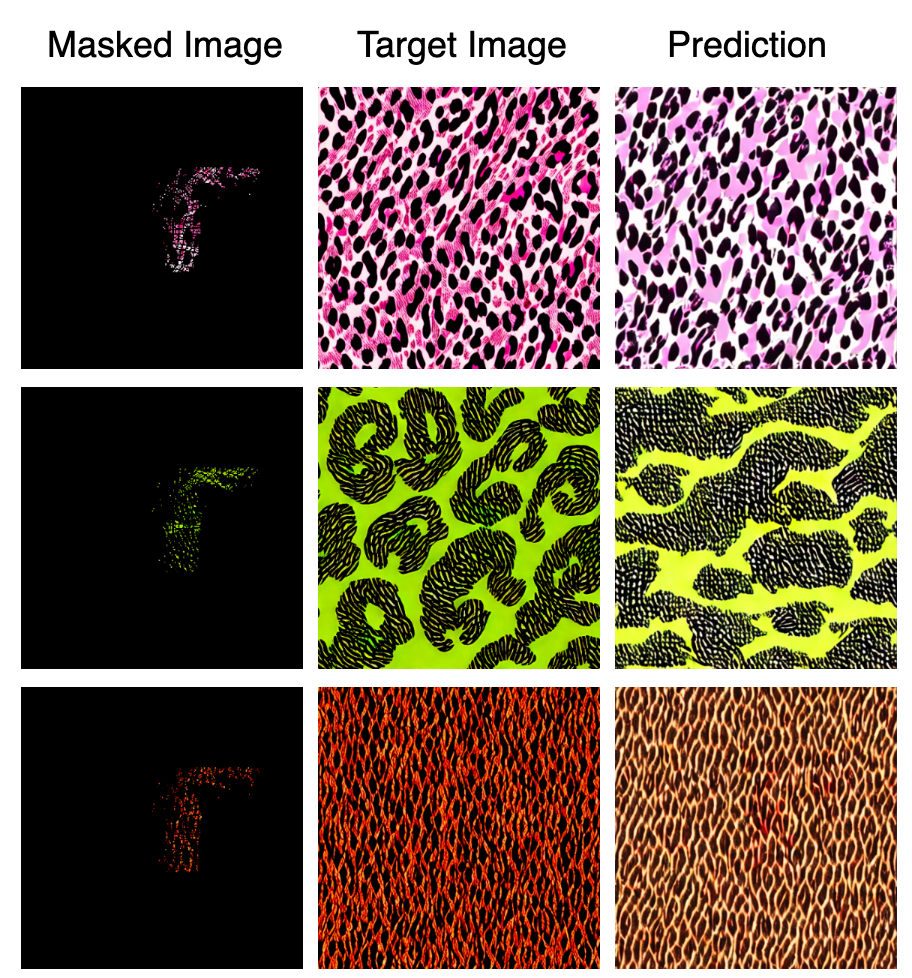
\includegraphics[width=0.47\textwidth]{figures/pbr_examples.png}
  \caption{\textbf{Example of Diffuse Texture Predictions.} The model predicts the diffuse texture based 
  on the observed partial masked image.}
  \label{fig:examples}
\end{figure}

There is an increasing interest in digitalising garments, that is, converting an image of a person wearing clothing into a 3D model 
of the depicted garments. In this work, we focus specifically on extracting high-quality physically based rendering (PBR) 
texture maps. In particular, we target three key components: diffuse, which captures the base color of the garment material; 
normal, which represents the surface orientation; and roughness, which characterizes the smoothness or roughness of the surface.

PBR texture maps are essential for realistic rendering of garment appearance and are thus of particular importance for downstream applications 
in gaming and the film industry. However, most existing methods extract only RGB texture maps, 
which include baked-in lighting from the original environment, limiting their adaptability and usefulness for other 
scenes or renderers.

Extracting high-quality PBR texture maps from a single RGB image poses several challenges. 
First, the problem involves modeling both the geometry and the appearance of the garment. 
Input images typically vary in lighting conditions and camera positions, making it difficult to disentangle material 
properties from illumination. In addition, garments themselves introduce domain-specific complications: 
self-occlusions often obscure parts of the fabric, which hinders accurate pattern capture; 
logos may be difficult to isolate and are frequently overlaid on the fabric in ways that complicate extraction; 
and finally, garment textures exhibit significant variation, ranging from simple, repetitive motifs to complex, 
irregular patterns.

Most prior work has concentrated on the geometry, while texture modeling is usually simplified to generating \textit{RGB} 
texture maps, as seen in methods such as \textit{Garment3DGen} \cite{garment3dgen}, \textit{DeepIron} \cite{deepiron}, 
or \textit{Wordrobe} \cite{WordRobe}. To the best of our knowledge, \textit{Fabric Diffusion} (FBD) \cite{fabricdiffusion} is 
the only method that directly attempts to generate PBR texture maps from a single image. 
However, this approach comes with limitations. FBD relies on a user-provided patch of the garment to model local 
texture patterns, assuming these can be seamlessly tiled to cover the surface. This assumption fails when patterns are not 
globally repetitive, and it may produce unnatural seams between tiles. 
Additionally, logo extraction in FBD requires the user to manually crop the logo, 
after which the model removes background and lighting artifacts. 
While effective in isolated cases, this process is impractical for full-garment digitalisation and does not 
generalise well to garments with multiple logos.

A further bottleneck in this field is the absence of a large-scale public dataset that pairs 
garment images with corresponding PBR texture maps. This data gap presents a key obstacle to 
training more robust and generalisable models for PBR texture extraction from images.

In this work, we take a first step toward scalable, fully-automated garment digitalization by addressing the 
task of UV-space texture inpainting. Given a partially observed diffuse texture map, our goal is to complete 
the garment appearance in UV space, and predict corresponding diffuse (Figure \ref{fig:examples}), normal and roughness 
texture maps. For simplicity, we do not address logo modeling.

To inform our method design, we conduct a systematic evaluation of key training and inference choices. 
We ask: (1) What are the optimal text and image guidance scales during inference? (2) What is the best initialization strategy for fine-tuning? (3) 
How do training set size and duration affect model performance?

We find that a text guidance scale of 1.5 and image scale of 5.0 yield the best results. 
Further, initializing from InstructPix2Pix and fine tuning the full model leads to the best performance. 
Surprisingly, we observe that training on only 5k images performs nearly as well as using the full 27k set, 
although longer training time consistently improves results.

We summarise our contributions as follows:
\begin{itemize}[itemsep=2pt, topsep=2pt]
  \item We introduce a new dataset of 27{,}000 PBR texture maps generated by a pre-trained DressCode \cite{dresscode} model.
  \item We propose a new method for UV-space texture inpainting that is trained on the proposed dataset.
  \item We conduct a systematic evaluation of key training and inference choices.
  \item We show that our method achieves the best performance on all metrics compare to the existing state-of-the-art inpainting methods.
\end{itemize}

All the code and data is available via the following link:
\url{https://bit.ly/garment-diffusion}.

\begin{figure*}[t]
  \centering
  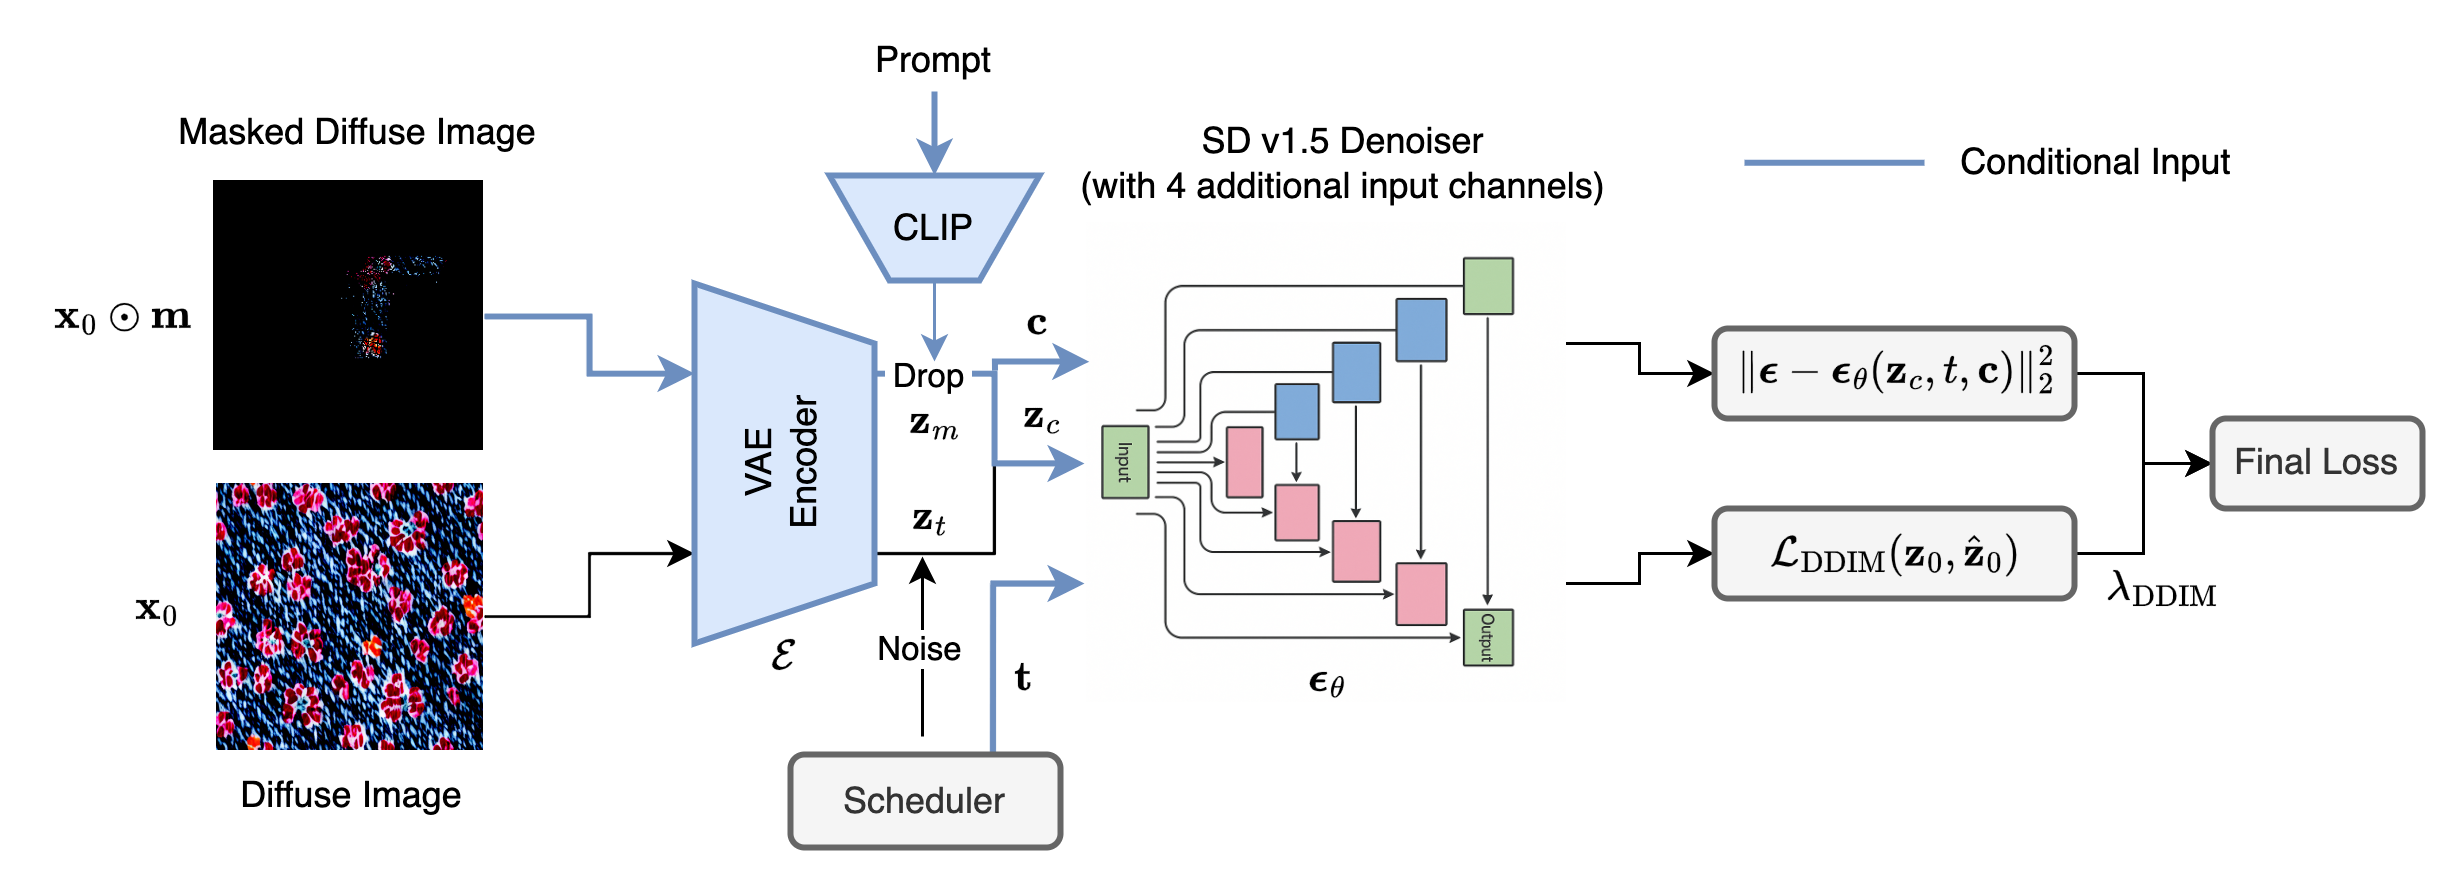
\includegraphics[width=1.0\textwidth]{figures/pbr_train_overview.png}
  \vspace{0.25em}
  \caption{\textbf{Overview of the Training Pipeline.} Inputs are first encoded into the latent space using a pre-trained (frozen) VAE and CLIP encoder. 
  A timestep $t$ is sampled via the PNDM scheduler, and noise is added to the target image latent. 
  The diffusion model is conditioned on the noisy latent, masked image latent, timestep, and text prompt. 
  It is trained to predict the added noise, with supervision from a weighted sum of MSE and DDIM reconstruction losses.}
  \label{fig:trn-overview}
\end{figure*}
\section{Related Work}

\textbf{General Material Texture Generation.} \textit{TexGen}~\cite{texgen} proposes a generative model for RGB texture synthesis in UV space, 
conditioned on either image or text inputs, and integrates 3D geometry information into the texture generation pipeline. 
\textit{Material Palette}~\cite{materialpalette} targets PBR material extraction from single images of 
real-world surfaces and introduces LoRA-based fine-tuning of diffusion models. 
\textit{DreamPBR}~\cite{dreampbr} and \textit{DreamMat}~\cite{dreammat} explore high-quality PBR texture generation from text, with the 
former supporting multi-modal inputs including fabric-related prompts. 
However, their models are either unpublished or lack garment-specific outputs such as normal maps. 
\textit{MatFusion}~\cite{matfusion} addresses the removal of baked-in lighting from input images for SVBRDF 
estimation and serves as a key component in \textit{FabricDiffusion}'s PBR extraction pipeline. Our work draws 
inspiration from these (e.g. considering using LoRA for finetuning) advances while focusing specifically on garment texture reconstruction.

\textbf{Garment Texture Generation.} \textit{FabricDiffusion}~\cite{fabricdiffusion} proposes a two-stage pipeline that first normalizes RGB garment textures 
and then employs an external model to predict the corresponding PBR texture maps, leveraging prior SVBRDF estimation techniques. 
\textit{Garment3DGen}~\cite{garment3dgen} introduces a multi-stage framework for 3D garment modeling, combining geometry and texture streams into a 
renderable output; however, it relies solely on RGB textures. Similarly, \textit{DeepIron}~\cite{deepiron} presents a pipeline involving garment segmentation, 
texture unwrapping, and inpainting, followed by application of the recovered texture onto a predefined sewing pattern, 
with its main novelty being the learned unwarping module. Our approach differs in focusing explicitly on recovering garment-specific diffuse texture maps for the 
entire garment (not just a patch like in \textit{FabricDiffusion}). 

\textbf{3D Garment Generation.}  
\textit{DressCode}~\cite{dresscode} introduces a multi-stage framework for text-driven garment 
synthesis, combining an autoregressive model that generates sewing patterns from prompts with 
a conditional diffusion model that produces corresponding PBR textures. 
\textit{WordRobe}~\cite{WordRobe} maps text inputs to textured 3D garments via a disentangled 
latent garment space and CLIP-based alignment, but produces only RGB textures. 
\textit{Design2Cloth}~\cite{design2cloth} enables mask-guided 3D garment generation and 
releases a large dataset of over 27{,}000 real-world garment scans. 
\textit{PICTURE}~\cite{picture} offers greater design flexibility by disentangling 
garment style and texture, employing a two-stage pipeline that first predicts garment shape
 and then generates texture conditioned on that shape. Finally, \textit{VTON360}~\cite{vton360} 
 addresses the challenge of viewpoint consistency in virtual try-on, introducing a method 
 for generating high-fidelity garments renderable from arbitrary angles.  
All these approaches focus on end-to-end 3D garment generation. 
In contrast, our method focuses specifically on high-quality \textit{texture reconstruction} 
from real images, aiming to recover physically meaningful material properties. 
As such, it can serve as a plug-in module for enhancing the realism and generalizability of 
generative pipelines that rely on RGB textures or simplified appearance models.


\begin{table*}[t]
  \centering
  \begin{subtable}[t]{0.48\textwidth}
    \vspace{0pt}
    \centering
    \begin{tabular}{l|ccc}
      \toprule
      \textbf{Model} & \textbf{LPIPS} $\downarrow$ & \textbf{SSIM} $\uparrow$ & \textbf{PSNR} $\uparrow$ \\
      \midrule
      Ours         & \textbf{0.45} & \textbf{0.17} & \textbf{13.04} \\
      Kandinsky 2.2 & 0.91 & 0.09 & 9.55 \\
      SD-Inpaint   & 0.97 & 0.02 & 6.56 \\
      Pix2Pix      & 1.00 & 0.03 & 6.36 \\
      SD           & 0.95 & 0.02 & 6.46 \\
      \bottomrule
    \end{tabular}
    \subcaption{Comparison to non-finetuned baselines.}
    \label{tab:best-vs-baseline}
  \end{subtable}
  \hfill
  \begin{subtable}[t]{0.48\textwidth}
    \vspace{0pt}
    \centering
    \begin{tabular}{cc|ccc}
      \toprule
      \textbf{TNS} & \textbf{TT [hrs]} & \textbf{LPIPS} $\downarrow$ & \textbf{SSIM} $\uparrow$ & \textbf{PSNR} $\uparrow$ \\
      \midrule
      27,000 & 30 & 0.50 & 0.16 & 12.41 \\
      \midrule
      27,000 & 60 & \textbf{0.45} & \textbf{0.17} & 13.04 \\
      5,000  & 30 & 0.49 & \textbf{0.17} & 13.11 \\
      15,000 & 30 & 0.50 & 0.16 & 13.10 \\
      20,000 & 30 & 0.51 & 0.17 & \textbf{13.12} \\
      10,000 & 30 & 0.52 & \textbf{0.17} & 12.65 \\
      \bottomrule
    \end{tabular}
    \subcaption{Effect of training set size and training time.}
    \label{tab:scale-study}
  \end{subtable}
  \caption{\textbf{Comparison to Non-Finetuned Baselines and Scale Study.}}
\end{table*}
\section{Method}

\textbf{Latent Diffusion Model}. We make use of a pre-trained VAE \cite{vae} encoder-decoder pair $(\mathcal{E}, \mathcal{D})$ 
for diffuse textures, where $\mathcal{E}: \mathbb{R}^{H \times W \times 3} \rightarrow \mathbb{R}^{C \times H' \times W'}$ 
encodes RGB images into a latent space, and $\mathcal{D}$ maps latents back to image space. 
The decoder was specifically fine-tuned for the task of reconstructing diffuse textures 
\cite{dresscode}.

Figure \ref{fig:trn-overview} shows an overview of our fine tuning pipeline. Given an input diffuse texture $\mathbf{x}_0$ and a binary mask $\mathbf{m}$, we encode the full and masked textures using the VAE encoder:
\begin{equation}
\mathbf{z}_0 = \mathcal{E}(\mathbf{x}_0), \quad \mathbf{z}_m = \mathcal{E}(\mathbf{x}_0 \odot \mathbf{m}),
\end{equation}

where $\odot$ denotes element-wise multiplication. We then sample a timestep $t \sim \mathcal{U}(1, T)$, using PNDM scheduler \cite{pndm}, and generate a noisy latent:
\vspace{0.0em}
\begin{equation}
\mathbf{z}_t = \sqrt{\bar{\alpha}_t} \mathbf{z}_0 + \sqrt{1 - \bar{\alpha}_t} \boldsymbol{\epsilon}, \quad \boldsymbol{\epsilon} \sim \mathcal{N}(0, \mathbf{I}),
\end{equation}

where $\bar{\alpha}_t$ is the cumulative product of noise schedule coefficients. We then concatenate the masked latent $\mathbf{z}_m$ and the noisy latent $\mathbf{z}_t$ to form the input to the diffusion model:
\begin{equation}
\mathbf{z}_c = [\mathbf{z}_m, \mathbf{z}_t]
\end{equation}

A conditioning text prompt $\mathbf{c}$ (constant across all samples) is embedded using CLIP 
\cite{clip}. To enable classifier-free guidance \cite{cfg}, we randomly drop the 
conditioning with some probability $p_{\text{drop}}$.

The model $\boldsymbol{\epsilon}_\theta$ is trained to predict the noise $\boldsymbol{\epsilon}$ added to $\mathbf{z}_0$. The total loss is then a weighted sum of the denoising objective and a DDIM reconstruction loss:
\begin{align}
  \mathcal{L} = \|\boldsymbol{\epsilon} - \boldsymbol{\epsilon}_\theta(\mathbf{z}_c, t, \mathbf{c})\|_2^2 
  \notag \\
  + \lambda_{\text{DDIM}} \cdot \mathcal{L}_{\text{DDIM}}(\mathbf{z}_0, \hat{\mathbf{z}}_0) \tag{4}
\end{align}
  
where $\hat{\mathbf{z}}_0$ is the model's reconstruction using DDIM inversion \cite{ddim} and $\lambda_{\text{DDIM}}$ is the weight of DDIM loss.

During inference, we adopt the same approach as in \textit{InstructPix2Pix} \cite{instructpix2pix}, 
where we condition the diffusion model on latents of the masked texture $\mathbf{z}_m$ and text prompt 
$\mathbf{z_c}$ to iteratively denoise from the noisy input image $\mathbf{z}_T$ to $\hat{\mathbf{z}}_0$. 
Importantly, we make use of classifier-free guidance \cite{cfg} to enable control over the text prompt and 
image guidance influence on the final texture. Based on our experiments, we find the text guidance scale $w_T = 1.5$ 
and image guidance scale $w_I = 5.0$ to be optimal. Using these guidance scales, we can express the classifier-free guidance as:
\vspace{0.0em}
\begin{align*}
  \tilde{\boldsymbol{\epsilon}}_{\theta}(\mathbf{z}_t, &\mathbf{c}_I, \mathbf{c}_T) = \boldsymbol{\epsilon}_{\theta}(\mathbf{z}_t, \varnothing, \varnothing) \\
  &\quad + w_I \cdot \left( \boldsymbol{\epsilon}_{\theta}(\mathbf{z}_t, \mathbf{c}_I, \varnothing) - \boldsymbol{\epsilon}_{\theta}(\mathbf{z}_t, \varnothing, \varnothing) \right) \tag{5} \\
  &\quad + w_T \cdot \left( \boldsymbol{\epsilon}_{\theta}(\mathbf{z}_t, \mathbf{c}_I, \mathbf{c}_T) - \boldsymbol{\epsilon}_{\theta}(\mathbf{z}_t, \mathbf{c}_I, \varnothing) \right)
\end{align*}


Finally, to map the predicted latent back to image space, we make use of texture specific pretrained 
decoder $\mathcal{D}$ adapted from \textit{DressCode} \cite{dresscode}.


\textbf{Data.} We generate a dataset of 27{,}000 PBR texture maps using pretrained DressCode \cite{dresscode} model. Specifically,
we first generate 30 different queries for colour, texture and pattern. We then feed each possible combination of these
queries to the DressCode model which then generates a corresponding PBR texture map.

% SD v1.5 (img2img)
% SSIM: 0.02430877275764942, PSNR: 6.464392185211182, LPIPS: 0.9525905251502991

% SD v1.5 inpaint (inpatient)
% SSIM: 0.020838197320699692, PSNR: 6.564342498779297, LPIPS: 0.9757870435714722

% kandinsky
% SSIM: 0.09910932183265686, PSNR: 9.545990943908691, LPIPS: 0.9103674292564392

% # valiant-resonance-120, before resume: final_eval/lpips=0.50461 final_eval/ssim=0.16205 final_eval/psnr=12.41427

\section{Results}
\begin{figure}[t]
  \centering
  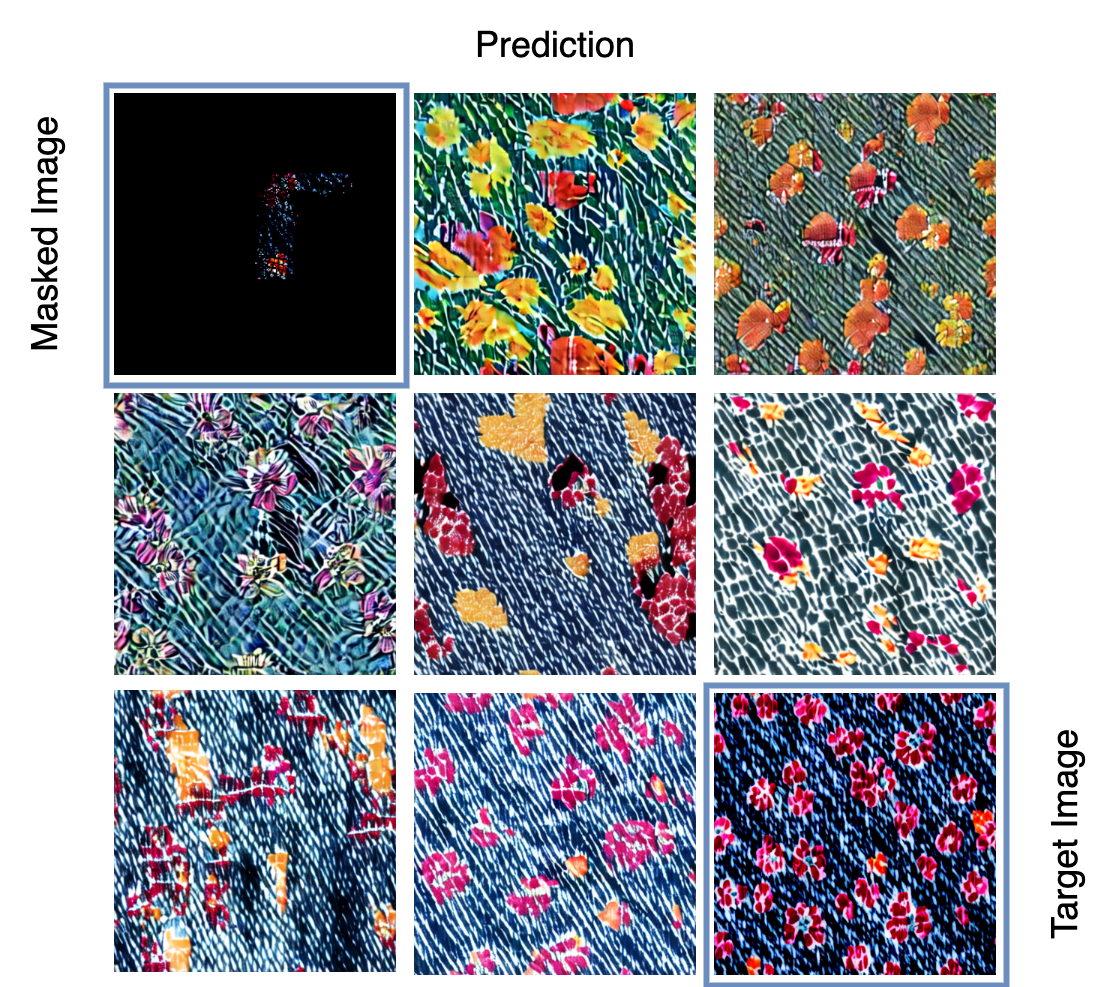
\includegraphics[width=0.45\textwidth]{figures/pbr_test_overview.png}
  \caption{\textbf{Evolution of the Best Model's Predictions.} 
  The model's predictions on a single validation sample over the training process. First prediction in the figure made 
  after 10,000 steps. The following predictions are made every 5,000 steps.}
  \label{fig:test-overview}
\end{figure}

\begin{table*}[t]
  \centering
    \begin{tabular}{ccccccc|ccc}
    \toprule
    \textbf{DDIM Weight} & \textbf{LR} & \textbf{BSZ} & \textbf{LoRA} & \textbf{Scratch} & \textbf{Inpaint} & \textbf{Base Model} & \textbf{LPIPS} $\downarrow$ & \textbf{SSIM} $\uparrow$ & \textbf{PSNR} $\uparrow$ \\
    \midrule
    0.50 & 1e-04 & 20 & \xmark & \xmark & \xmark & sd & \textbf{0.50} & \textbf{0.16} & \textbf{12.41} \\
    \midrule
    0.50 & 1e-04 & 40 & \cmark & \xmark & \xmark & pix2pix & 0.57 & 0.09 & 11.75 \\
    0.50 & 1e-05 & 20 & \xmark & \cmark & \xmark & sd & 0.82 & 0.02 & 7.48 \\
    \midrule
    0.75 & 1e-04 & 20 & \cmark & \xmark & \cmark & sd-inpaint & 0.96 & 0.13 & 9.25 \\

    \bottomrule
    \end{tabular}
    \caption{\textbf{Ablation Study Over Model Architecture and Training Strategy.} 
    All models trained for 30 hours on 27,000 samples. Best results per metric are highlighted in bold. 
    Top row shows the best model for reference.}
    \label{tab:arch-ablation}
\end{table*}

\vspace{1.5em}

\begin{table*}[t]
  \centering
  \begin{tabular}{cc|cccc}
    \toprule
    \textbf{Text Scale} & \textbf{Image Scale} & \textbf{LPIPS Rank} & \textbf{SSIM Rank} & \textbf{PSNR Rank}  & \textbf{Mean Rank} \\
    \midrule
    5.0 & 2.5 & \textbf{6.0} & 7.0 & \textbf{5.0}  & \textbf{6.00} \\
    1.5 & 5.0 & 9.0 & 4.0 & 6.0 & 6.33 \\
    2.5 & 7.5 & 10.0 & \textbf{2.0} & 9.0 & 7.00 \\
    \bottomrule
  \end{tabular}
  \caption{\textbf{Guidance Scale Ranking.} 
  The best performing configuration is highlighted in bold. 
  The table shows the rank of each configuration on SSIM, PSNR, and LPIPS.}
  \label{tab:guidance-ranking}
\end{table*}

\vspace{-2.0em}
\subsection{Experimental Setup}
Our best model is trained on a single NVIDIA V100 GPU for 60 hours using a batch size of 20. 
We optimize using the AdamW optimizer with a learning rate of \(1 \times 10^{-4}\), 
a weight decay of \(1 \times 10^{-2}\), and 1000 warm-up steps. 
To stabilize training, we apply gradient clipping based on the \(\ell_2\)-norm. 
Input images are used at their original resolution of \(512 \times 512\) pixels. 
The DDIM loss is scaled by a factor of 0.5. Training is performed on the full dataset comprising 27{,}000 samples, 
with validation conducted every 1000 steps on a held-out set of 300 images. 
During inference, we employ a guidance scale of 1.5 for text and 5.0 for the input image. 
Our finetuning is initialized from the Stable Diffusion v1.5 checkpoint \cite{sd} to which we add additional input channels
for the masked image. Since we use a pre-trained \textit{frozen} decoder to map predicted latents 
back to image space, we report image quality metrics - SSIM, LPIPS, and PSNR-based 
solely on the predicted diffuse texture maps. We assume that the model achieving the 
best performance on diffuse textures will also generalize best to the full set of PBR texture maps.

\subsection{Best Model Performance}
Table~\ref{tab:best-vs-baseline} compares our best performing model with non-finetuned SOTA baselines. 
Our method outperforms all baselines across all metrics. Figure~\ref{fig:test-overview} illustrates the model's 
prediction trajectory on a validation sample throughout training. While the model successfully captures the overall 
structure and color distribution, it struggles to recover fine-grained texture details. 
These results highlight the importance of task-specific finetuning. The following subsections analyze the impact of 
key hyperparameters on model performance.


\subsection{Guidance Scale During Inference}
\vspace{-.8em}

Diffusion models are sensitive to the guidance scale hyperparameters, which can significantly impact output quality. 
We evaluate the effect of varying text and image guidance scales over the grid {1.5, 2.5, 5.0, 7.5, 10.0}, resulting 
in 25 configurations. For each, we run inference on 100 validation samples using our best model and compute 
standard image quality metrics. Each configuration is ranked per metric, with rank 1 denoting the best. 
As shown in Table~\ref{tab:guidance-ranking}, the best-performing setting uses a text scale of 5.0 and an image scale of 2.5. 
However, we select the second-best configuration (text: 1.5, image: 5.0) to emphasize image guidance, which is more aligned 
with the task.

\subsection{Training Set Size and Duration}

Table~\ref{tab:scale-study} presents the impact of training set size and training duration on model performance. 
As expected, using the full dataset and training for more iterations yields the best results. 
However, the performance differences are relatively small—even when training on just 5,000 samples. 
We hypothesize that this may stem from limited diversity in the dataset, which was generated by another model, 
though we leave this question for future investigation.

\begin{figure}[t]
  \centering
  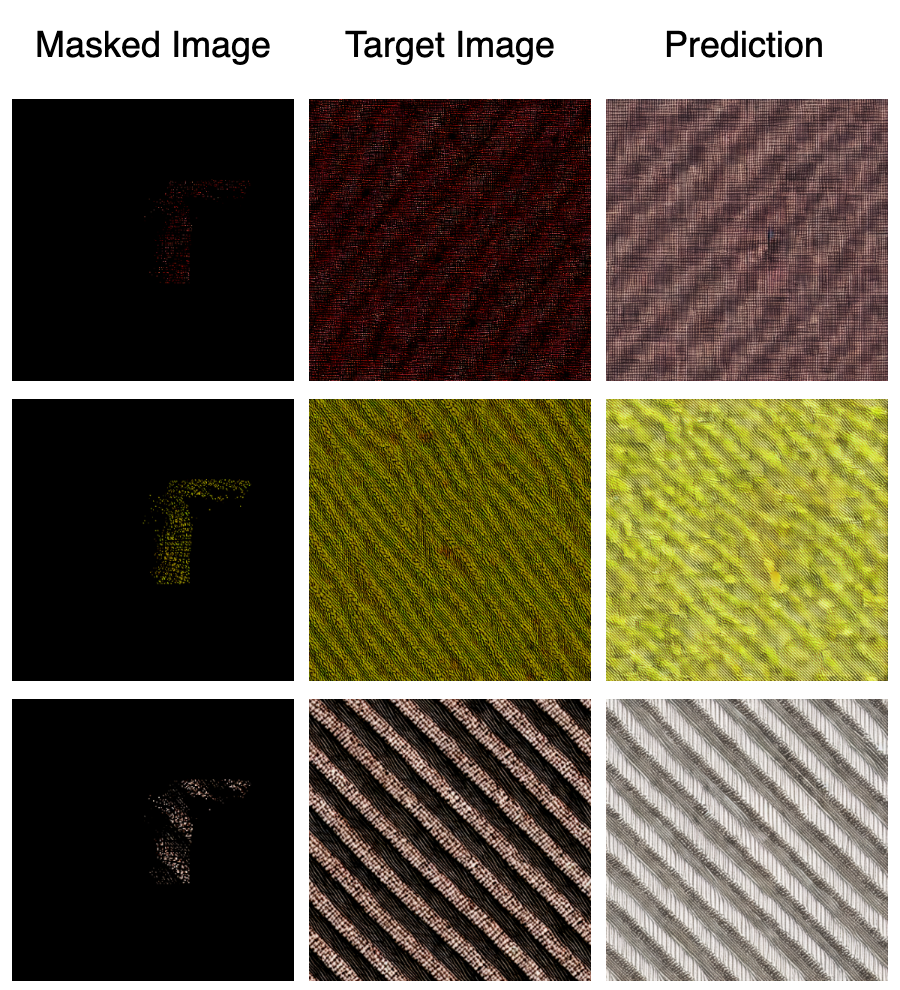
\includegraphics[width=0.43\textwidth]{figures/failure_cases.png}
  \caption{\textbf{Hardest Cases.} Hardest cases based on SSIM metric for the best model.}
  \label{fig:hardest-cases}
\end{figure}


\subsection{Training Strategy and Architecture}

Finetuning the full Stable Diffusion v1.5 model, which contains over one billion parameters, 
is computationally demanding. We therefore explore alternative strategies: finetuning only LoRA weights, training a smaller model 
from scratch, and initializing from an inpainting model. As shown in Table~\ref{tab:arch-ablation}, full-model finetuning yields 
the best performance. While LoRA~\cite{lora} enables the use of larger batch sizes, 
it results in a measurable drop in quality. Training from scratch performs significantly worse, 
highlighting the critical role of pretraining. Surprisingly, finetuning from an inpainting model also underperforms. 
Unlike InstructPix2Pix, which conditions on the masked image, noise, and text prompt, the inpainting model additionally uses the binary mask as 
input. Our qualitative analysis suggests that this model tends to fill only the masked garment region while leaving 
surrounding areas untouched, limiting its effectiveness for global texture refinement.


\subsection{Optimisation Hyperparameters}

\begin{table}[t]
  \centering
  \begin{tabular}{ccc|ccc}
  \toprule
  \textbf{W} & \textbf{LR} & \textbf{Sch.} & \textbf{LPIPS} $\downarrow$ & \textbf{SSIM} $\uparrow$ & \textbf{PSNR} $\uparrow$ \\
  \midrule
  0.50 & 1e-04 & \xmark & \textbf{0.45} & \textbf{0.16} & \textbf{12.41} \\
  0.75 & 1e-05 & \xmark & 0.58 & 0.14 & 12.21 \\
  0.25 & 1e-05 & \xmark & 0.63 & 0.12 & 12.08 \\
  0.50 & 1e-05 & \cmark & 0.69 & 0.12 & 10.70 \\
  0.50 & 1e-05 & \xmark & 0.69 & 0.09 & 9.88 \\
  0.00 & 1e-05 & \xmark & 0.78 & 0.06 & 10.07 \\
  0.50 & 3e-06 & \xmark & 0.83 & 0.09 & 10.22 \\
  \bottomrule
  \end{tabular}
  \caption{\textbf{Comparison of Hyperparameter Configurations.} 
  The best performing configuration is highlighted in bold. For a 
  fair comparison, all models are trained for 30 hours on 27,000 samples. Results are sorted by LPIPS, SSIM and PSNR (in that order).}
  \label{tab:hyperparams}
\end{table}



Table~\ref{tab:hyperparams} reports the impact of different hyperparameter configurations on model performance. 
We find that increasing the learning rate from $1\text{e}{-5}$ to $1\text{e}{-4}$ leads to the most significant improvement. 
Additionally, raising the DDIM loss weight from 0.50 to 0.75 yields further performance gains.

\subsection{Hardest Cases}

Figure~\ref{fig:hardest-cases} presents the lowest-performing cases based on SSIM for the 
best model. The model typically struggles with accurate color reproduction (e.g., last row) 
or fails to recover fine textures (e.g., middle row). We attribute this to the limited 
information in the masked input image, which requires the model to rely heavily on 
learned priors over the garment texture distribution. This is a challenging task, 
especially when trained on synthetic data.

\subsection{Full PBR Texture Maps Prediction}

During inference, the model predicts a complete set of PBR texture maps from a single masked input image. As illustrated in Figure~\ref{fig:full-pbr-showcase}, the predicted normal and roughness maps closely match the ground truth, while the diffuse texture exhibits noticeable deviations in color. Table~\ref{tab:full-pbr-metrics} confirms this trend, showing stronger performance for normal and roughness prediction compared to diffuse. We attribute this discrepancy to the higher variability and ambiguity inherent in diffuse textures. Unlike normals and roughness, which are locally smooth and strongly constrained by shading cues, the diffuse map often contains high-frequency patterns and color variations that are harder to infer and continue into the masked regions.

\section{Future Work \& Limitations}
In this work, all models were trained using the diffuse texture map as the sole supervision target in 
latent space. We hypothesize, however, that incorporating additional supervision from the normal and 
roughness maps could further enhance the model's performance on these components. 
We leave this for future investigation.

Moreover, our results suggest that strong performance can be achieved with a relatively small training set, 
indicating that limited dataset diversity, rather than size, may be the primary bottleneck. 
An important avenue for future research is evaluating the model's ability to generalize to real-world images. In this context, pretrained models such as Fabric Diffusion~\cite{fabricdiffusion} could be used to synthesize more realistic PBR supervision signals.

Finally, our evaluation was conducted using a single predefined mask. Future work should explore the 
model's robustness to a wider range of masking patterns, including unseen or irregular occlusions.


\begin{figure}[t]
  \centering
  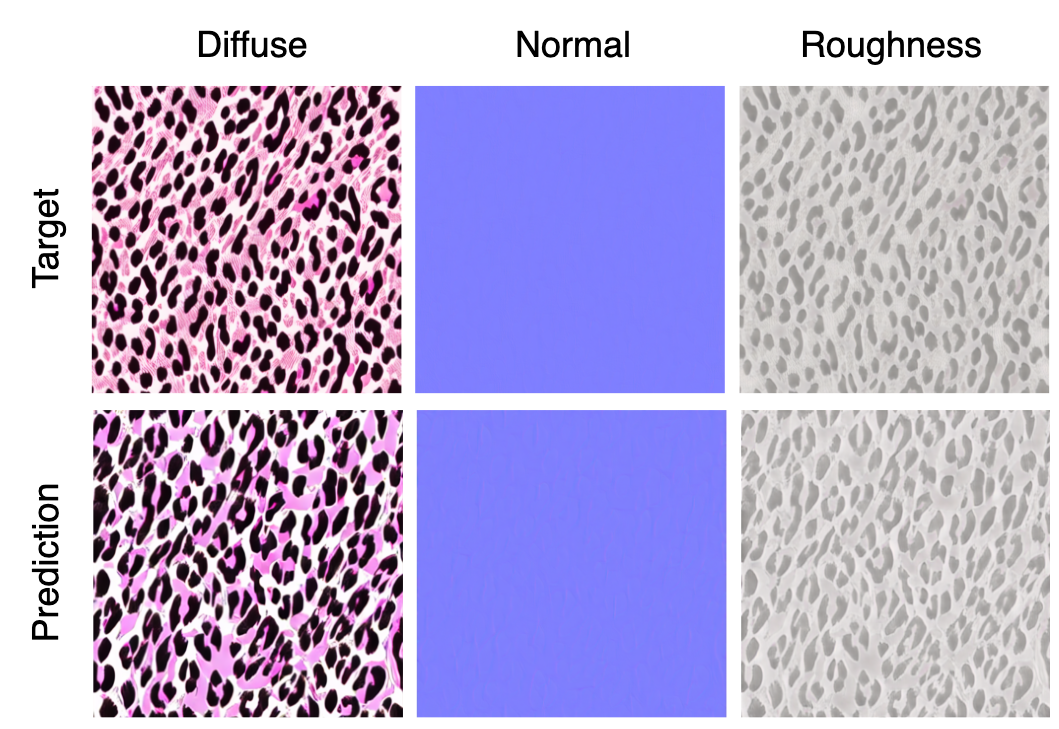
\includegraphics[width=0.45\textwidth]{figures/full_pbr_showcase.png}
  \caption{\textbf{Full PBR texture maps prediction.} Showcase of the best model's prediction of a full set of PBR texture maps 
  based on a single masked image.}
  \label{fig:full-pbr-showcase}
\end{figure}

\begin{table}[t]
  \centering
  \begin{tabular}{l | ccc | c}
    \toprule
    \textbf{Metric} & \textbf{Diffuse} & \textbf{Normal} & \textbf{Roughness} & \textbf{Mean} \\
    \midrule
    LPIPS $\downarrow$ & 0.45 & 0.26 & 0.28 & 0.33 \\
    SSIM $\uparrow$ & 0.17 & 0.50 & 0.52 & 0.40 \\
    PSNR $\uparrow$ & 13.04 & 25.76 & 23.63 & 20.81 \\
    \bottomrule
    \end{tabular}
  \caption{\textbf{Evaluation metrics for diffuse, normal, and roughness maps.} 
  The best model's performance on predicting a full set of PBR texture maps.}
  \label{tab:full-pbr-metrics}
\end{table}


\section{Conclusion}
We presented a method for predicting PBR texture maps from a single masked image. 
By fine-tuning a pre-trained Stable Diffusion v1.5~\cite{sd} on a synthetic dataset of 
27,000 PBR textures, our approach produces high-quality results and outperforms state-of-the-art 
inpainting models that are not fine-tuned for this task. Notably, we demonstrate that comparable 
performance can be achieved even when training on a small subset of the dataset, and that 
extended training time consistently improves results.

Additionally, we find that full-model fine-tuning yields substantially better performance than using LoRA, 
and that fine-tuning an inpainting model underperforms compared to using the 
InstructPix2Pix~\cite{instructpix2pix} pipeline.

Future work should investigate the model's generalization to real-world images and explore the benefits 
of incorporating additional supervision from normal and roughness maps to enhance performance on these 
texture components. Another promising direction is studying the role of the mask in shaping the model's 
effectiveness and robustness.

\section{Acknowledgements}
I would like to thank my supervisor, Yingxuan You, for her valuable feedback and guidance throughout the semester. 
Further, I would like to thank to Prof. Fua for hosting me in his lab and providing me with the computational resources.


\newpage
\bibliographystyle{plainnat}
\bibliography{references}

\end{document}